\subsection{Experimental Methodology and Results}
In the following paragraphs, we report the methodology and results of our experiments.

\subsubsection{RQ1. Mono-objective SBSE Validation}
\paragraph{Method}

To answer the first research question RQ1, we conduct a mono-objective search for compiler optimization exploration in order to evaluate the non-functional properties of optimized code. Thus, we generate optimization sequences using three search-based techniques (Random Search RS, GA, and NS) and compare their performance results to standard GCC optimization levels (O1, O2, O3 and Ofast). 
In this experiment, we choose to optimize for execution time (S), memory usage (MR), and CPU consumption (CR). Each non-functional property is improved separately and independently of other metrics. We recall that other properties can be also optimized using NOTICE (e.g., code size, compilation time, etc.), but in this experiment, we focus only on three properties.
\vspace{-1em}
\begin{figure}[h]
	\centering
	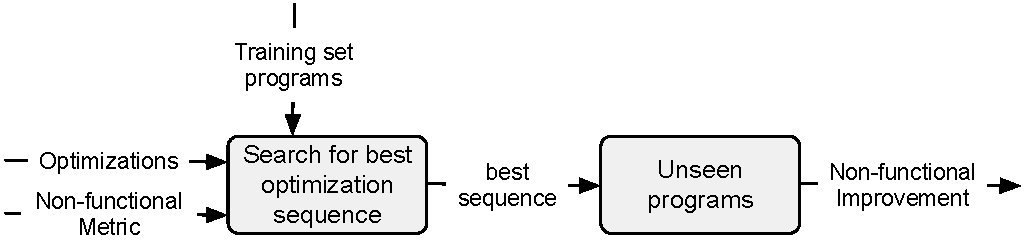
\includegraphics[width=1.\linewidth]{Ressources/sensitivity.pdf}
	\caption{Evaluation strategy to answer RQ1 and RQ2}
	
\end{figure}

\setlength\abovecaptionskip{0.25ex}
As it is shown on the left side of Figure 5, given a list of optimizations and a performance objective, we use NOTICE to search for the best optimization sequence across a set of input programs that we call \textit{"the training set"}. Then, we generate a set of random Csmith programs \textit{"the training set"} (10 programs) and apply generated sequences to these programs. Therefore, the code quality metric, in this setting, is equal to the average performance improvement (S, MR, or CR) and that, for all programs under test. 

%while p
%the goal of this initial experiment is to: (1) evaluate the effectiveness of our component-based infrastructure to extract non-functional properties such as memory and CPU consumptions; (2) evaluate the performance of our proposed diversity-based exploration of optimization sequences (NS) to GA and RS; and finally (3) find the optimal solution relative to the input training set.

%The goal of this experiment is to show that NOTICE is able to generate 





\paragraph{Results}


\vspace{-1.2em}
%\iffalse
\begin{table}[h]
	\centering
	\caption{Results of mono-objective optimizations}
	\label{my-label}
	\begin{tabular}{|l|l|l|l|l|l|l|c|}
		\hline
		& \textbf{O1}                    & \textbf{O2}                    & \textbf{O3}                    & \textbf{Ofast}                 & \textbf{RS}                    & \textbf{GA}                    & 
		\textbf{NS} \\
		\hhline{|=|=|=|=|=|=|=|=|}
		S  &  1.051 & 1.107  & 1.107  & 1.103  & 1.121  &  1.143 &  1.365  \\ \hline
		MR(\%) & 4.8  & -8.4  &  4.2 & 6.1  &  10.70 & 15.2  &  15.6  \\ \hline
		CR(\%) & -1.3  & -5  & 3.4  & -5  &  18.2 & 22.2  &  23.5  \\ \hline
	\end{tabular}
\end{table}
%\fi
%-NS better than 3 algos\\
%-conflicting results for standard levels
%The goal of this first experiment is to compare the performance improvement of novelty-based generated sequences to standard GCC optimizations and to RS and GA.  
Table 3 reports the comparison results of three non-functional properties CR, MR, and S. At the first glance, we can clearly see that all search-based algorithms outperform standard GCC levels with minimum improvement of 10\% for memory usage and 18\% for CPU time (when applying RS). 
Our proposed NS approach has the best improvement results for three metrics with 1.365 of speedup, 15.6\% of memory reduction and 23.5\% of CPU time reduction across all programs under test. NS is clearly better than GA in terms of speedup. However, for MR and CR, NS is slightly better than GA with 0.4\% improvement for MR and 1.3\% for CR. RS has almost the lowest optimization performance but is still better than standard GCC levels.

We remark as well that applying standard optimizations has an impact on the execution time with a speedup of 1.107 for O2 and O3. Ofast has the same impact as O2 and O3 for the execution speed. However, the impact of GCC levels on resource consumption is not always efficient. O2, for example, increases resource consumption compared to O0 (-8.4\% for MR and -5\% for CR). This can be explained by the fact that standard GCC levels apply some aggressive optimizations that increase the performance of generated code and deteriorate system resources.  
%Thus, NOTICE can clearly provide an alternative to catch most relevant optimization sequence regarding resource consumptions.
 	
%This agrees to the idea that standard optimizations mdoes not produce always
%the same impact results on resource consumption and may be highly dependent on the benchmark and the source code they have been tested on.
 %Using O2, we find that the memory consumption has increased by almost 8.4\% compared to the baseline. Same findings for CR when applying O1, O2 and Ofast. 



\noindent\fbox{\parbox{\linewidth-2\fboxrule-2\fboxsep}{
		\textbf{Key findings for RQ1.} \\
-- Best discovered optimization sequences using mono-objective search techniques always provide better results than standard GCC optimization levels.\\
-- Novelty Search is a good candidate to improve code in terms of non-functional properties since it is able to discover optimization combinations that outperform RS and GA.  }}
\\
\subsubsection{RQ2. Sensitivity}
\paragraph{Method}
Another interesting experiment is to test the sensitivity of input programs to compiler optimizations and evaluate the general applicability of best optimal optimization sets, previously discovered in RQ1. These sequences correspond to the best generated sequences using NS for the three non-functional properties S, MR and CR (i.e., sequences obtained in column 8 of Table 3). 
Thus, we apply best discovered optimizations to new unseen Csmith (100 new random programs) and we compare then, the performance improvement across these programs (see right-hand side of Figure 5). We also apply standard optimizations, O2 and O3, to new Csmith programs in order to compare the performance results.
The idea of this experiment is to test whether new generated Csmith programs are sensitive to previously discovered optimizations or not. 
%If so, then compiler users and researchers can use NOTICE to auto-tune compilers and build optimizations for their input programs. 
%in order to build general optimization sequences from their representative
If so, this will be useful for compiler users and researchers to use NOTICE in order to build general optimization sequences from their representative \textit{training set} programs.
\vspace{-1.2em}
\begin{figure}[h]
	\centering
	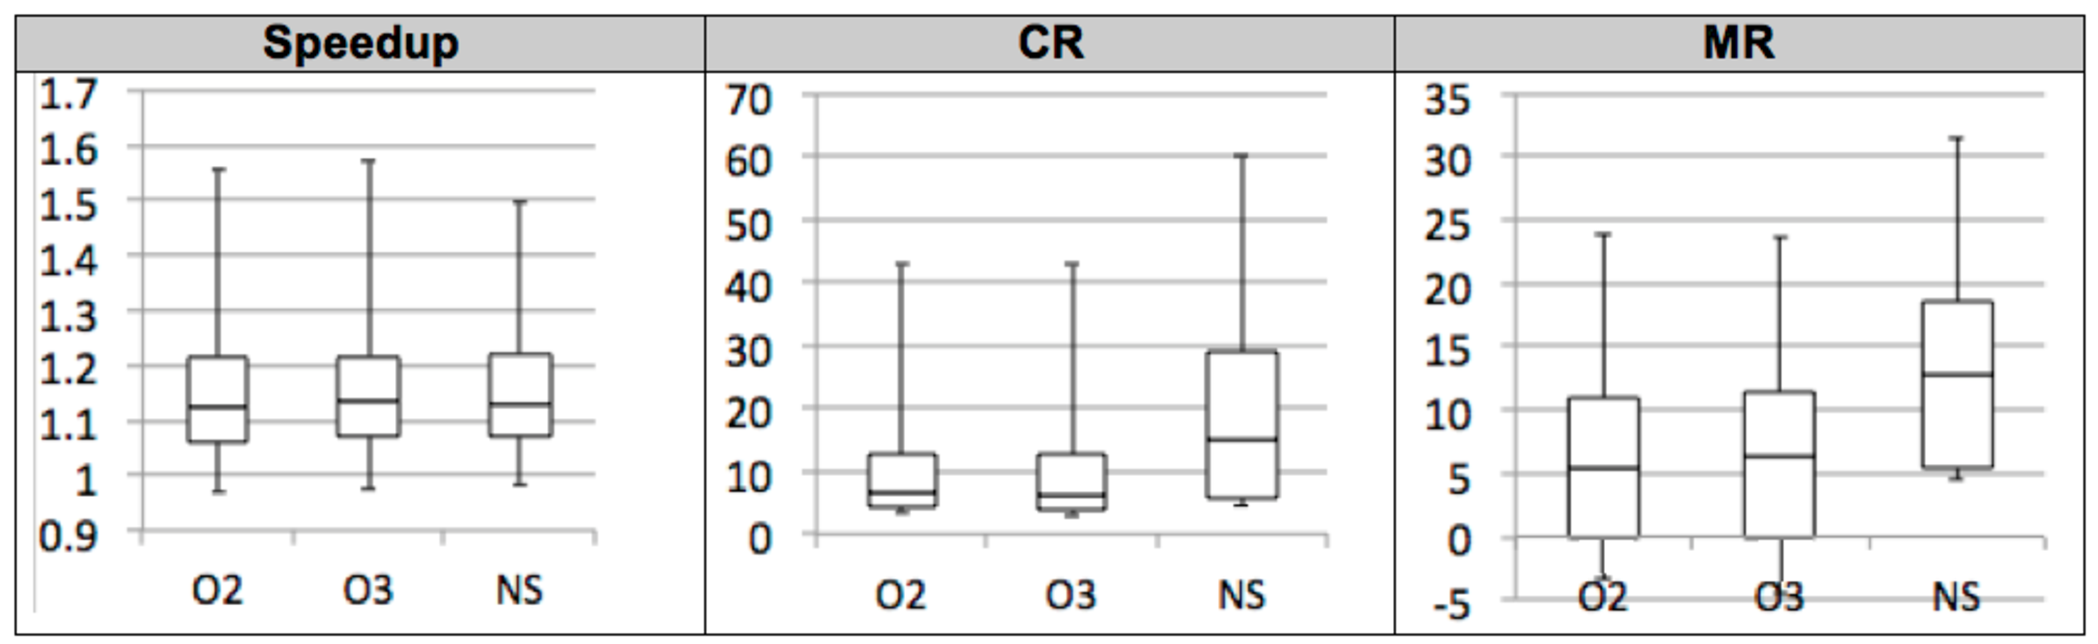
\includegraphics[width=1.\linewidth]{Ressources/box.pdf}
	\caption{Boxplots of the obtained performance results across 100 unseen Csmith programs, for each non-functional property: Speedup (S), memory (MR) and CPU (CR) and for each optimization strategy: O2, O3 and NS}
\end{figure}
\paragraph{Results}
Figure 6 shows the distribution of memory, CPU and speedup improvement across new Csmith programs. For each non-functional property, we apply O2, O3 and best NS sequences. Speedup results show that the three optimization strategies lead to almost the same distribution with a median value of 1.12 for speedup. This can be explained by the fact that NS needs too long  to find the sequence that best optimizes the execution speed. Meanwhile, O2 and O3 have also the same impact on CR and MR which is almost the same for both levels (CR median value is 8\% and around 5\% for MR).
However, the impact of applying best generated sequences using NS clearly outperforms O2 and O3 with almost 10\% of CPU improvement and 7\% of memory improvement. This proves that NS sequences are efficient and can be used to optimize resource consumption of new Csmith programs. This result also proves that Csmith code generator applies the same rules and structures to generate C code. For this reason, applied optimization sequences always have a positive impact on the non-functional properties.


\noindent\fbox{\parbox{\linewidth-2\fboxrule-2\fboxsep}{
		\textbf{Key findings for RQ2.}\\
	-- It is possible to build general optimization sequences that perform better than standard optimization levels \\
	-- Best discovered sequences in RQ1 can be mostly used to improve the memory and CPU consumption of Csmith programs. To answer RQ2, Csmith programs are sensitive to compiler optimizations.}}\\
\subsubsection{RQ3. Impact of optimizations on resource usage}
\paragraph{Method}
In this experiment, we use NOTICE to provide an understanding of optimizations behavior, in terms of resource consumption, when trying to optimize for execution time. Thus, we choose one instance of obtained results in RQ1 related to the best speedup improvement (i.e., results obtained in line 1 of Table 3) and we study the impact of speedup improvement on memory and CPU consumption. We also compare resource usage data to standard GCC levels as they were presented in Table 3. Improvements are always calculated over the non-optimized version. The idea of this experiment is to: (1) prove, or not, the usefulness of involving resource usage metrics as key objectives for performance improvement; (2) the need, or not, of multi-objective search strategy to handle both resource usage and performance properties.

%In this experiment, we apply standard optimizations and different mono-objective heuristics individually to 5 Cbench programs and use NOTICE to profile applications in terms of resource usage.  

%To answer RQ3, we choose one instance of obtained results in RQ1 related to the best improvement in terms of execution time (i.e., where NS had the best speedup) and we study the impact of performance improvement on memory and CPU consumption. 
%Following again a mono-objective approach, we try in this experiment to maximize the speedup \textit{S} per-benchmark and study, at the same time, the impact of speedup \textit{S} on resource consumption namely memory footprint and CPU usage. 
%In this experiment, we apply standard optimizations and different mono-objective heuristics individually to 5 Cbench programs and use NOTICE to profile applications in terms of resource usage.   
%The goal of this experiment is to: (1) use NOTICE infrastructure to provide an understanding of optimizations behavior, in terms of resource consumption, when trying to optimize for execution time; (2) prove the usefulness of resource consumption reduction as a key objective for performance improvement.

\paragraph{Results}

%\begin{figure}[h]
%	\centering
%	\includegraphics[width=1.\linewidth]{Ressources/infra_novelty_stat2.png}
%	\caption{Evaluating the speedup after applying standard optimization options compared to best generated optimization using NS}
%\end{figure}
Figure 7 shows the impact of speedup optimization on resource consumption. For instance, O2 and O3 that led to the best speedup improvement among standard optimization levels in RQ1, present opposite impact on resource usage. Applying O2 induces -8.4\% of MR and -5\% of CR. However, applying O3 improves MR and CR respectively by 3.4\% and 4.2\%. Hence, we note that when applying standard levels, there is no clear correlation between speedup and resource usage since compiler optimizations are generally used to optimize the execution speed and never evaluated to reduce system resources.
On the other hand, the outcome of applying different mono-objective algorithms for speedup optimization also proves that resource consumption is always in conflict with execution speed. The highest MR and CR is reached using NS with respectively 1.2\% and 5.4\%. This improvement is considerably low compared to scores reached when we have applied resource usage metrics as key objectives in RQ1 (i.e., 15.6\% for MR and 23.5\% for CR). Furthermore, we note that generated sequences using RS and GA have a high impact on system resources since all resource usage values are worse than the baseline.
These results agree to the idea that compiler optimizations do not put too much emphasis on the trade-off between execution time and resource consumption.

%Thus, NOTICE can clearly provide an alternative to catch most relevant optimization sequence regarding resource consumptions.

%This agrees to the idea that standard optimizations mdoes not produce always
%the same impact results on resource consumption and may be highly dependent on the benchmark and the source code they have been tested on.
%Using O2, we find that the memory consumption has increased by almost 8.4\% compared to the baseline. Same findings for CR when applying O1, O2 and Ofast. 
\noindent\fbox{\parbox{\linewidth-2\fboxrule-2\fboxsep}{
		\textbf{Key findings for RQ3.} \\
		-- Optimizing software performance can induce undesirable effects on system resources.\\
		-- A trade-off is needed to find a correlation between software performance and resource usage.
	}}
 
\subsubsection{RQ4. Trade-offs between non-functional properties}
\paragraph{Method}
Finally, to answer RQ4, we use NOTICE again to find trade-offs between non-functional properties. In this experiment, we choose to focus on the trade-off \textit{$<$ExecutionTime--MemoryUsage$>$}. In addition to our NS adaptation for multi-objective optimization, we implement a commonly used multi-objective approach namely NSGA-II~\cite{deb2002fast}. We denote our NS adaptation by \textit{NS-II}. We recall that NS-II is not a multi-objective approach as NSGA-II. It uses the same NS algorithm. However, in this experiment, it returns the optimal Pareto front solutions instead of returning one optimal solution relative to one goal. 
Apart from that, we apply different optimization strategies to assess our approach. 
\begin{figure}[h]
	\centering
	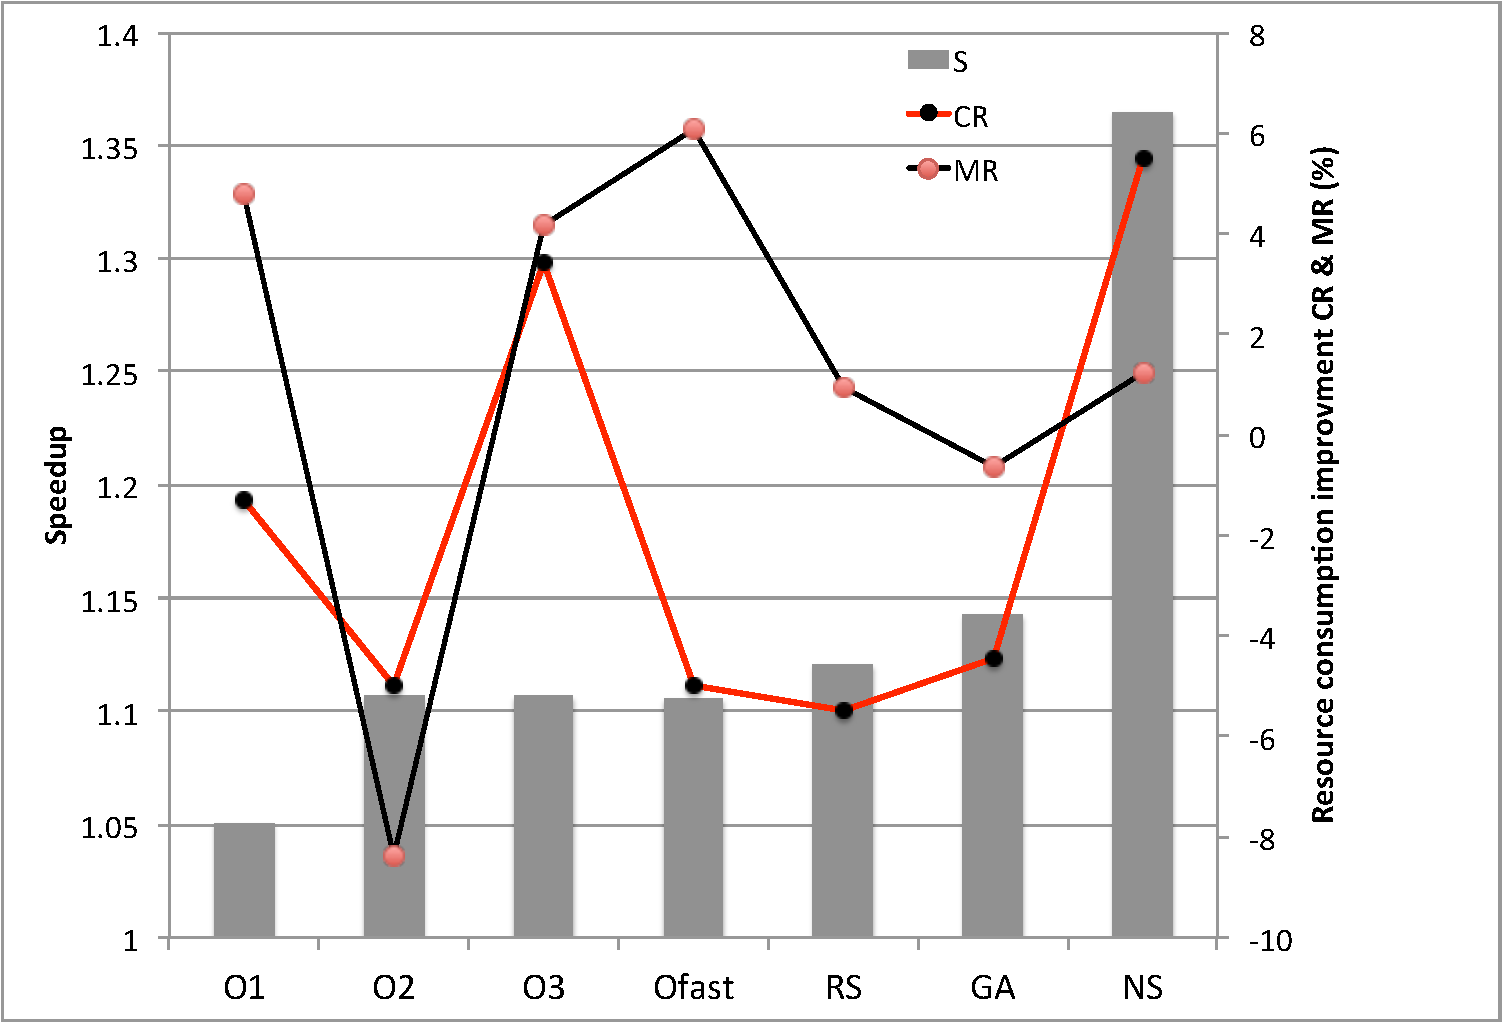
\includegraphics[width=0.9\linewidth]{Ressources/rq3.pdf}
	\caption{Impact of speedup improvement on memory and CPU consumption for each optimization strategy}
\end{figure}

First, we apply standard GCC levels. Second, we apply best generated sequences relative to memory and speedup optimization (the same sequences that we have used in RQ2). Thus, we denote by \textit{NS-MR} the sequence that yields to the best memory improvement MR and \textit{NS-S} to the sequence that leads to the best speedup. This is useful to compare mono-objective solutions to new generated ones.



In this experiment, we assess the efficiency of generated sequences using only one Csmith program.
We evaluate the quality of the obtained Pareto optimal optimization based on raw data values of memory and execution time. Then, we compare qualitatively the results by visual inspection of the Pareto frontiers.
The goal of this experiment is to check whether it exists, or not, a sequence that can reduce both execution time and memory usage.
%We report the comparison results of our NS adaptation for optimizations generation to the current state-of-the-art multi-objective approaches namely NSGA-II. 

%Two tradeoffs are investigated in this section; $<$execution time--memory usage$>$ and $<$execution time--CPU usage$>$.


\paragraph{Results}
Figure 8 shows the Pareto optimal solutions that achieved the best performance assessment for the trade-off \textit{$<$ExecutionTime--MemoryUsage$>$}. The horizontal axis indicates the memory usage in raw data (in Bytes) as it is collected using NOTICE. In similar fashion, the vertical axis shows the execution time in seconds. Furthermore, the figure shows the impact of applying standard GCC options and best NS sequences on memory and execution time. Based on these results, we can see that NSGA-II performs better than NS-II. In fact, NSGA-II yields to the best set of solutions that presents the optimal trade-off between the two objectives. Then, it is up to the compiler user to use one solution from this Pareto front that satisfies his non-functional requirements (six solutions for NSGA-II and five for NS-II). For example, he could choose one solution that maximizes the execution speed in favor of memory reduction. On the other side, NS-II is capable to generate only one non-dominated solution. For NS-MR, it reduces as expected the memory consumption compared to other optimization levels. The same effect on execution time when applying the best speedup sequence NS-S. We also note that all standard GCC levels are dominated by our different heuristics NS-II, NSGA-II, NS-S and NS-MR.
This agrees to the claim that standard compiler levels do not present a suitable trade-off between execution time and memory usage.


\begin{figure}[h]
	\centering
	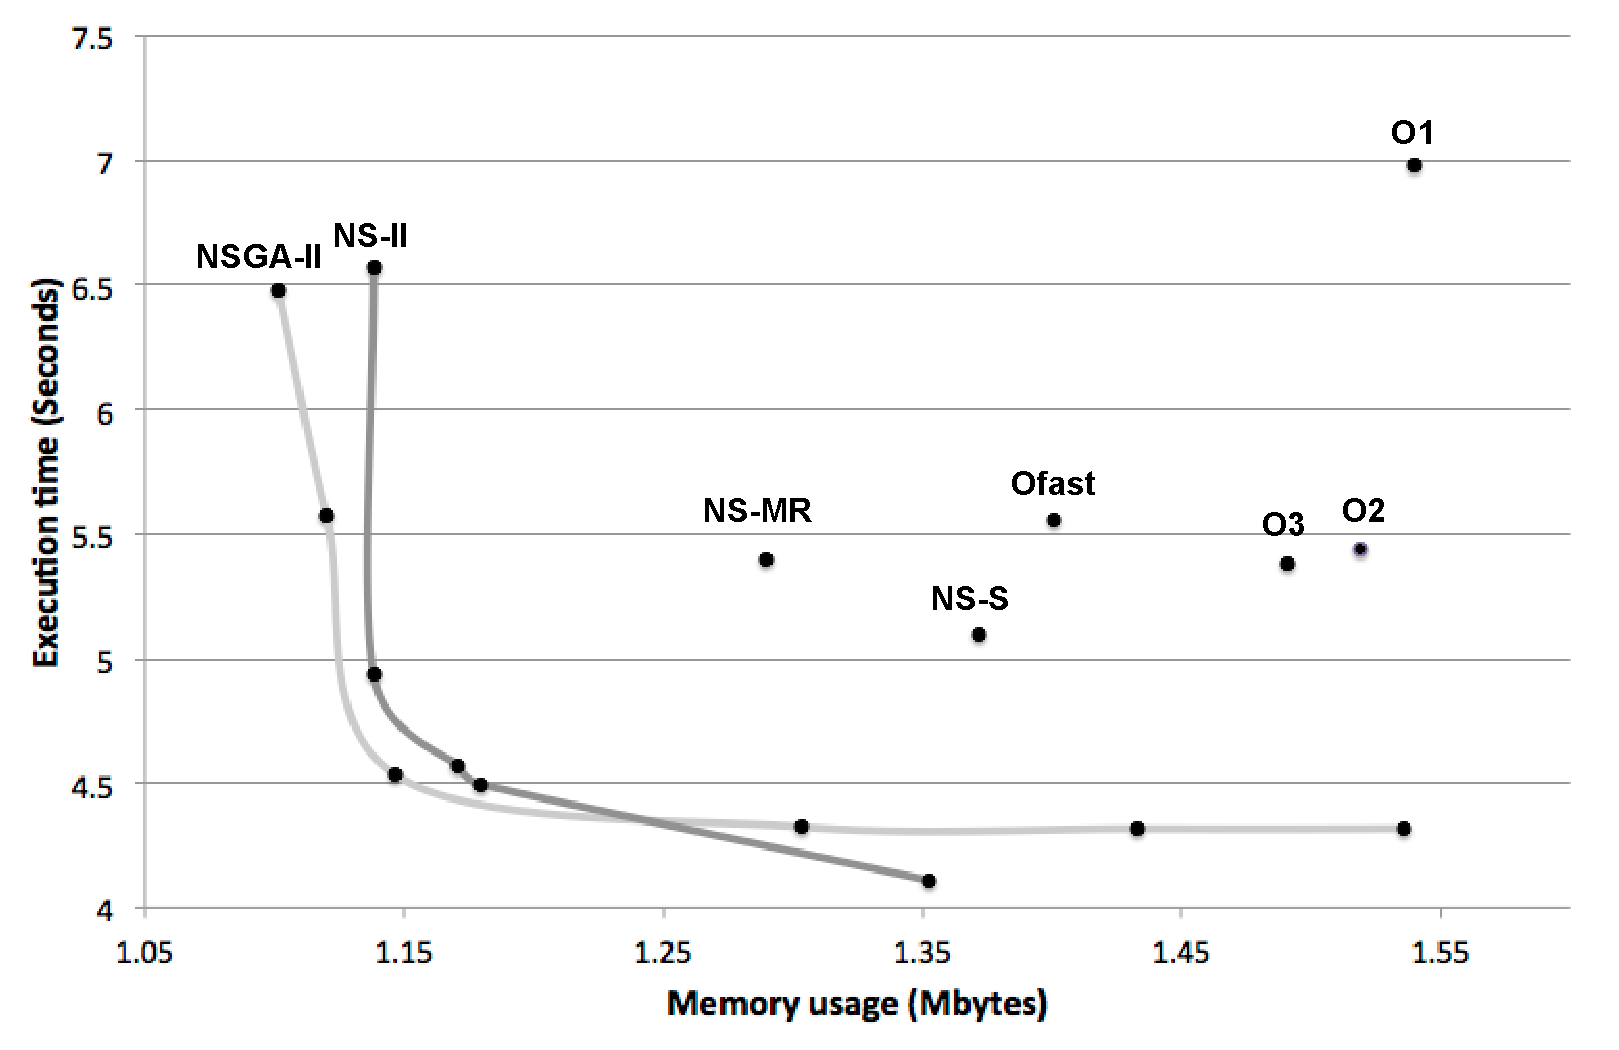
\includegraphics[width=0.9\linewidth]{Ressources/pareto.pdf}
	\caption{Comparison results of obtained Pareto fronts using NSGA-II and NS-II}
\end{figure}


\noindent\fbox{\parbox{\linewidth-2\fboxrule-2\fboxsep}{
		\textbf{Key findings for RQ4.} \\
-- NOTICE is able to construct optimization levels that represent optimal trade-offs between non-functional properties. \\
-- NS is more effective when it is applied for mono-objective search. \\
-- NSGA-II performs better than our NS adaptation for multi-objective optimization. However, NS-II performs clearly better than standard GCC optimizations and previously discovered sequences in RQ1.
}}
\subsection{Discussions}
Through these experiments, we showed that NOTICE is able to provide facilities to compiler users to test the non-functional properties of generated code. It provides also a support to search for the best optimization sequences through mono-objective and multi-objective search algorithms. NOTICE infrastructure has shown its capability and scalability to satisfy user requirements and key objectives in order to produce efficient code in terms of non-functional properties. During all experiments, standard optimization levels have been fairly outperformed by our different heuristics. 
Moreover, we have also shown (in RQ1 and RQ3) that optimizing for performance may be, in some cases, greedy in terms of resource usage. For example, the impact of standard optimization levels on resource usage is not always efficient even though it leads to performance improvement. 
Thus, compiler users would use NOTICE to test the impact of optimizations on the non-functional properties and build their specific sequences by trying to find trade-offs among these non-functional properties (RQ4). We would notice that for RQ1, experiments take about 21 days to run all algorithms. This run time might seem long but, it should be noted that this search can be conducted only once, since in RQ2 we showed that best gathered optimizations can be used with unseen programs of the same category as the training set, used to generate optimizations. This has to be proved with other case studies. As an alternative, it would be great to test model-based code generators. In the same fashion as Csmith, code generators apply to same rules to generate new software programs. Thus, we can use NOTICE to define general-purpose optimizations from a set of generated code artifacts. 
Multi-objective search as conducted in RQ4, takes about 48 hours, which we believe is acceptable for practical use. Nevertheless, speeding up the search speed may be an interesting feature for future research.
%good performance to detect most of the existing antipatterns, which
%could be very helpful to provide advice to both service clients and
%providers on the quality of their Web services.




%speeding up the search process may be an interesting avenue for future research.
\subsection{Threats to Validity}
Any automated approach has limitations. We resume, in the following paragraphs, external and internal threats that can be raised:
 
\textit{External validity} refers to the generalizability of our findings. In this study, we perform experiments on random programs using Csmith and we use iterative compilation techniques to produce best optimization sequences. We believe that the use of Csmith programs as input programs is very relevant because compilers have been widely tested across Csmith programs~\cite{chen2016empirical,yang2011finding}. Csmith programs have been used only for functional testing, but not for non-functional testing. However, we cannot assert that the best discovered set of optimizations can be generalized to industrial applications since optimizations are highly dependent on input programs and on the target architecture. In fact, experiments conducted on RQ1 and RQ2 should be replicated to other case studies to confirm our findings; and build general optimization sequences from other representative training set programs chosen by compiler users.

\textit{Internal validity} is concerned with the causal relationship between the treatment and the outcome. Meta-heuristic algorithms are stochastic optimizers, they can provide different results for the same problem instance from one run to another. Are we providing a statistically sound method or it is just a random result? Due to time constraints, we run all experiments only once. Following the state-of-the-art approaches in iterative compilation, previous research efforts~\cite{hoste2008cole,martinez2014multi} did not provide statistical tests to prove the effectiveness of their approaches. This is because experiments are time-consuming. However, we can deal with these internal threats to validity by performing at least five independent simulation runs for each problem instance. 
 
 
\iffalse
\begin{table}[]
	\centering
	\caption{My caption}
	\label{my-label}
	\begin{tabular}{@{}|l|c|c|c|c|c|c|c|c|c|c|c|c|c|c|c|c|c|c|c|c|@{}}
		\toprule
		\multirow{2}{*}{} & \multicolumn{2}{c|}{CB1} & \multicolumn{2}{c|}{CB2} & \multicolumn{2}{c|}{CB3} & \multicolumn{2}{c|}{CB4} & \multicolumn{2}{c|}{CB5} & \multicolumn{2}{c|}{CS1} & \multicolumn{2}{c|}{CS2} & \multicolumn{2}{c|}{CS3} & \multicolumn{2}{c|}{CS4} & \multicolumn{2}{c|}{CS5} \\ \cmidrule(l){2-21} 
		& Ox & Best & Ox & Best & Ox & Best & Ox & Best & Ox & Best & Ox & Best & Ox & Best & Ox & Best & Ox & Best & Ox & Best \\ \midrule
		Execution Speedup & \begin{tabular}[c]{@{}c@{}}4\%\\ (O3)\end{tabular} &  &  &  &  &  &  &  &  &  &  &  &  &  &  &  &  &  &  &  \\ \midrule
		Memory & \begin{tabular}[c]{@{}c@{}}4\%\\ (O3)\end{tabular} &  &  &  &  &  &  &  &  &  &  &  &  &  &  &  &  &  &  &  \\ \midrule
		CPU & \begin{tabular}[c]{@{}c@{}}4\%\\ (O3)\end{tabular} &  &  &  &  &  &  &  &  &  &  &  &  &  &  &  &  &  &  &  \\ \midrule
		Compilation Speedup &  &  &  &  &  &  &  &  &  &  &  &  &  &  &  &  &  &  &  &  \\ \midrule
		Code Size &  &  &  &  &  &  &  &  &  &  &  &  &  &  &  &  &  &  &  &  \\ \bottomrule
	\end{tabular}
\end{table}
\fi


 

